\documentclass{standalone}
\usepackage{fontspec}
\setsansfont{DejaVuSans.ttf}[Path=./,Kerning=Off,Ligatures={TeXOff,NoCommon}]
\usepackage{tikz}
\begin{document}
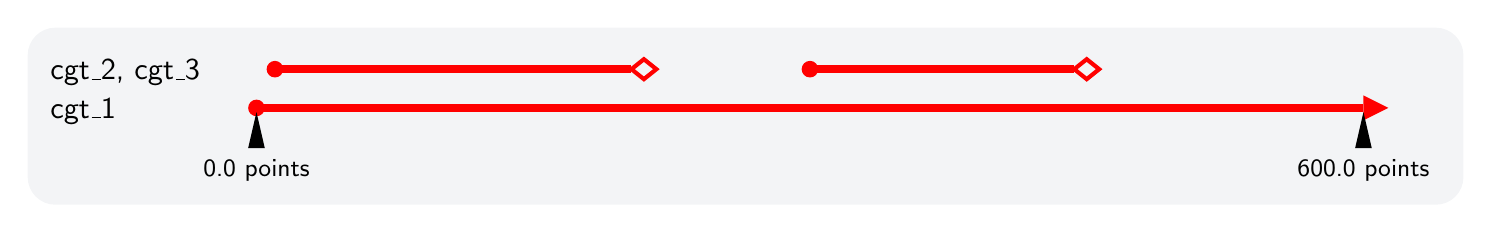
\begin{tikzpicture}[x=1pt,y=1pt,miter limit=4,font=\sffamily]
\definecolor{ts000000}{HTML}{000000}
\definecolor{tsF3F4F6}{HTML}{F3F4F6}
\definecolor{tsFF0000}{HTML}{FF0000}
\begin{scope}[shift={(16,16)}]
\path[rounded corners=10pt,fill=tsF3F4F6] (0,0) rectangle (518.8105,63.9766);
\path[draw=tsFF0000,line width=3pt] (82.6768,34.9766) -- (482.6768,34.9766);
\path[fill=tsFF0000] (82.6768,34.9766) circle[radius=3];
\path[fill=tsFF0000] (491.6768,34.9766) -- (482.6768,39.4766) -- (482.6768,30.4766) -- cycle;
\path[draw=tsFF0000,line width=3pt] (89.3434,48.9766) -- (218.1768,48.9766);
\path[fill=tsFF0000] (89.3434,48.9766) circle[radius=3];
\path[draw=tsFF0000,line width=1.5pt] (218.1768,48.9766) -- (222.6768,52.5766) -- (227.1768,48.9766) -- (222.6768,45.3766) -- cycle;
\path[draw=tsFF0000,line width=3pt] (282.6768,48.9766) -- (378.1768,48.9766);
\path[fill=tsFF0000] (282.6768,48.9766) circle[radius=3];
\path[draw=tsFF0000,line width=1.5pt] (378.1768,48.9766) -- (382.6768,52.5766) -- (387.1768,48.9766) -- (382.6768,45.3766) -- cycle;
\path[fill=ts000000] (82.6768,33.4766) -- (79.6768,20.4766) -- (85.6768,20.4766) -- cycle;
\path[fill=ts000000] (482.6768,33.4766) -- (479.6768,20.4766) -- (485.6768,20.4766) -- cycle;
\node[anchor=base west,inner sep=0,font=\sffamily\fontsize{11}{12.8047}\selectfont,text=ts000000] at (8,45.1685) {cgt\_2, cgt\_3};
\node[anchor=base west,inner sep=0,font=\sffamily\fontsize{11}{12.8047}\selectfont,text=ts000000] at (8,31.1685) {cgt\_1};
\node[anchor=base,inner sep=0,font=\sffamily\fontsize{9}{10.4766}\selectfont,text=ts000000] at (82.6768,10.1226) {0.0 points};
\node[anchor=base,inner sep=0,font=\sffamily\fontsize{9}{10.4766}\selectfont,text=ts000000] at (482.6768,10.1226) {600.0 points};
\end{scope}
\end{tikzpicture}
\end{document}
